\documentclass[12pt]{report}
\usepackage[utf8]{inputenc} 
\usepackage[T1]{fontenc}
\usepackage{layout}
\usepackage{graphicx}

%page de garde 
\title{Technical Report of the First Phase of the Project}
\author{Pierre-Yves Hervo \\Polytech Nantes High school of Engineering }
\date{11th  of July 2013}

\begin{document}
\maketitle

\begin{abstract}
This report explain how I managed to interface Praat and Java and how the Genetic Algorithm is implemented. The first part of this report will be an overAll to explain general concepts and the second part will deals with my particular Java implementation.

Important: This solution is working on windows 7, it is supposed to work on Linux but it wont work on a Mac because of the Praat's API.

\end{abstract}

\tableofcontents

\part{Overall}

\chapter{About the Genetic Algorithm}
This chapter deals with the basics of how my genetic algorithm work. I will explain it in detail in the second part with the explanations of my code.

\section{Principle}
The best way to recognise a vowel is to compare the formants of the candidate sound to the formants of a well known sounds.

For example, if we want to know if a sound is a "i", we will compare the formants of the candidate sound to the values which are defined for a i.

\section{The target}
As I said earlier, the values will be values for both frequency and bandwidth of two formants of a well known vowel. But this value are just a definition, in practice, we can estimate that a formant value can increase or decrease over 10\% of this value. So the fitness function of my GA compare the values of the formants of the candidate to the +/-10\% values of the target formants.

\section{The candidate}
We will compare the candidates formants to the reference formants. But for that purpose, we need to synthesise the sound and calculate its formants. The software Praat will do both for us. We need to send him parameters. The problem of how to send it parameters will be solved in the next chapter.

We need to send it values for each parameter representing a vocal element. See figure n bidule. Fortunately, Praat will automaticly complete the values for some parameters by default, so on the 49 parameters, we only need to define 20. So the element we will make evolve as a candidate will be sequence of possible values for this 20 parameters.


\chapter{How to connect Java and Praat}
Giving the Praat's API, we need to use two different ways to connect Java and Praat.
We need to consider one way to communicate between Java and Praat to send and execute the Praat script and another to send the response from Praat to Java.

\section{From Java to Praat}
We want to send a Praat's script to Praat and have it executed. The way I choose is the software SendPraat\cite{ref}. It is a program developed by the same authors as Praat. It allow to send orders to a {\bfseries running instance of Praat}\footnote{This is very important, if there is no Praat already launched, SendPraat won't work.}.
It means we need two programs :

\begin{enumerate}
\item a normal Praat software already launched.
\item SendPraat which will give it orders. No need to launch this one, it only works in command line.
\end{enumerate}

If you give SendPraat the name of a script, it will made Praat launch and execute it. The only thing left is to make Java executed SendPraat. For this, I used the Java Runtime Environment which can use the command line of windows. I will explain it in the second part of this report.

 and praat link in bibliography+ url

Note : I used a SendPraat.exe as I used windows but you can compile the source code yourself to use it in your own operating system. If you want to make Praat communicate with a C program, you can use the SendPraat directive, no need to compile source code. For more information, look at the Praat's API, section Praat scripting. As I was working in Java, the solution I presented is currently the best.

\section{From Praat to Java}
There is only one way to make Praat communicate with another program, whenever the language is, the sockets\footnote{It only work for windows and Linux, it is the Praat API wich manage it like this.}. 

Sockets are a way use in computer science to make two different program communicated. For this, they will use the network principles and send network packets to a computer on a specified port. It is not necessary that it was another computer, it can be the same and int that case, we use a local network call localhost. The first program will send a message to the other specifying the port and the second one will listen will listen to the port and get the message when it arrived.

Praat allows to send sockets by the directive "sendsocket" but it cant received sockets from another program. That is why we got to use the SendPraat program in the other side.
If Praat send a socket then our GA will need a functionality which always listen to this port and  will take the message. Such functionality basically call a {\bfseries Server}.
In that purpose, I implement a Java server that listen to a specific port. I will describe it in the second part of the report.

\section{Recap}
So in conclusion we had to consider two different side for the communications : the message from Java to Praat and the message from praat to Java. On the first side, we had to use a specific praat program called SendPraat and on the other side we had to use a Java's Server to listen to Praat's sockets.

The figure below show how it works :
\begin{figure}
\begin{center}
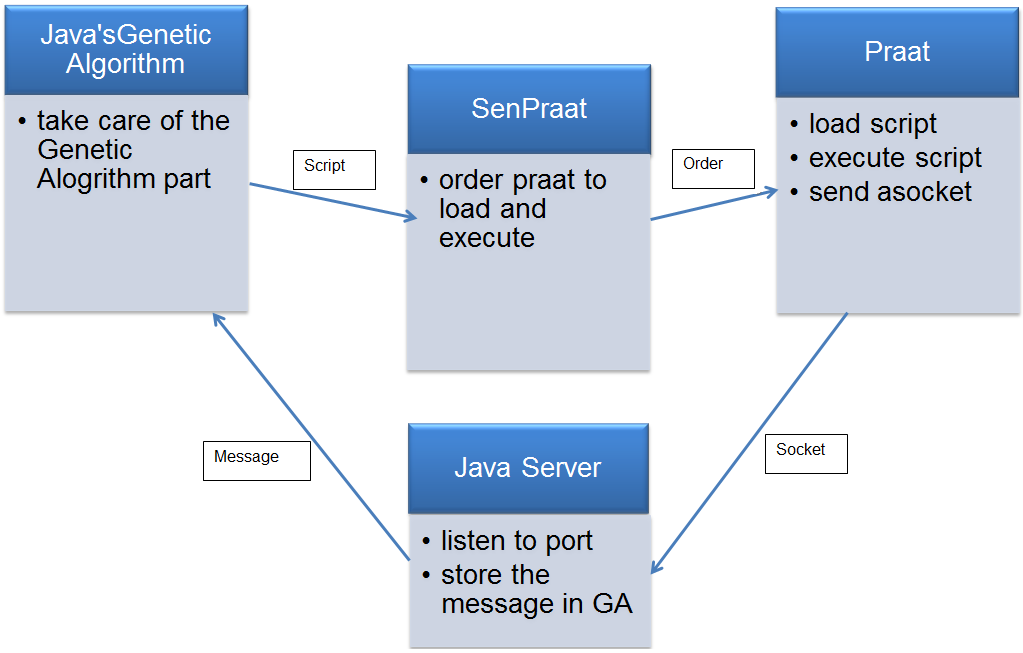
\includegraphics[scale=0.6]{resources/architecture.png} 
\end{center}
\caption{The exchange of information between Java and Praat and the role of each entity}
\label{ImageHumanVoice}
\end{figure}


\part{Implementation Details}
\chapter{the GA}
\section{watchmaker}
\section{basics elements to manipulate}
\section{the result}

\chapter{the communication}
\section{call to sendPraat}
\section{the server}
\appendix
\chapter{A scheme}

\listoffigures
\listoftables

\bibliographystyle{unsrt} 
\bibliography{bib} % mon fichier de base de données s'appelle bibli.bib
\end{document}